\documentclass[A4]{article}
\usepackage{amsmath}
\usepackage{listingsutf8}
\lstset{literate={č}{{\v c}}1 {š}{{\v s}}1 {ž}{{\v z}}1} %Paket listings (oz. listingsutf8) direktno ne podpirata šumnikov.
\lstset{basicstyle=\ttfamily, language=Octave} %Nastavimo, da je privzet jezik za lstlistings octave.
\usepackage[pdftex]{graphicx}
\usepackage[slovene]{babel} % slovenske nastavitve (naslovi, deljenje besed ...)
\usepackage[T1]{fontenc}    % font encoding; T1 podpira slovenščino
\usepackage[utf8]{inputenc} % input encoding; lahko je tudi [cp1250] ali [latin2]

\begin{document}
\title{Presek dveh implicitno danih premic}
\author{Janez Novak}
\maketitle
\section{Naloga}
Poiskati želimo presek dveh premic v ravnini, ki sta dani z enačbama
\[
	ax + by + c = 0 \ \textrm{ in } \ dx + ey + f = 0 \textrm{. }
\]

\section{Rešitev}
\subsection{Postopek reševanja}
Presek dveh nevzporednih premic je točka $T(x_0, y_0)$, kjer $x_0$ in $y_0$ rešita sistem linearnih enačb
\begin{align*}
	ax + by + c &= 0 \textrm{, }\\
	dx + ey + f &= 0 \textrm{, }
\end{align*}
ki predstavljata enačbi obeh premic.
Če zapišemo 
\[
	A = \begin{bmatrix} a & b \\ d & e \end{bmatrix} \ \textrm{ in } \ \mathbf{b} = -\begin{bmatrix} c \\ f \end{bmatrix} \textrm{, }
\]
potem iščemo rešitev $\mathbf{x} = [x_0, y_0]^\mathsf{T}$ sistema
\[
	A \mathbf{x} = \mathbf{b} \textrm{. }
\]
Premici se sekata v točki, če ima ta sistem eno samo rešitev, kar se zgodi natanko takrat, ko je $A$ polnega ranga oziroma $\det(A) \neq 0$. 
Ko $A$ ni polnega ranga, sta premici ali vzporedni ali pa naši podatki niso smiselni.

\subsection{Implementacija v {\sf octave}}
V {\sf octave}-u bomo rešitev poiskali z uporabo operatorja \lstinline!\!.
Vhodne podatke shranimo v matriko \lstinline!A! in vektor \lstinline!b! kot
zgoraj, nato pa poiščemo presečišče s klicem \lstinline!x = A\b!. Posebej moramo
obravnavati primer, ko $A$ ni polnega ranga, saj nam sicer operator
\lstinline!\! vrne rešitev po metodi najmanjših kvadratov. Zadostoval bo en
pogojni stavek: V primeru, da je $\det(A)$ primerljiva s strojno natančnostjo,
izpišemo napako.

Koda funkcije {\tt presecisce.m} brez testov je na koncu poročila.
Oglejmo si primer uporabe. Za premici $p : x + y - 1 = 0$ in $q : 2x - 3y + 2 = 0$ vnesemo:
\begin{lstlisting}
octave:1> p = [1, 1, -1];
octave:2> q = [2, -3, 2];
\end{lstlisting}
V $T$ shranimo koordinate presečišča:
\begin{lstlisting}
octave:3> T = presecisce(p, q);
\end{lstlisting}
in vse skupaj narišemo:
\begin{lstlisting}
octave:4> ezplot(@(x, y) p(1)*x + p(2)*y + p(3), [-2, 2])
octave:5> hold on 
octave:6> ezplot(@(x, y) q(1)*x + q(2)*y + q(3), [-2, 2])
octave:7> plot(T(1), T(2), 'o')
\end{lstlisting}
in sliko shranimo v datoteko:
\begin{lstlisting}
octave:8> print -dpdf slika.pdf  
\end{lstlisting}
Dobimo izris kot na sliki~\ref{slika:presek_premic}.
\begin{figure}
	\centering
	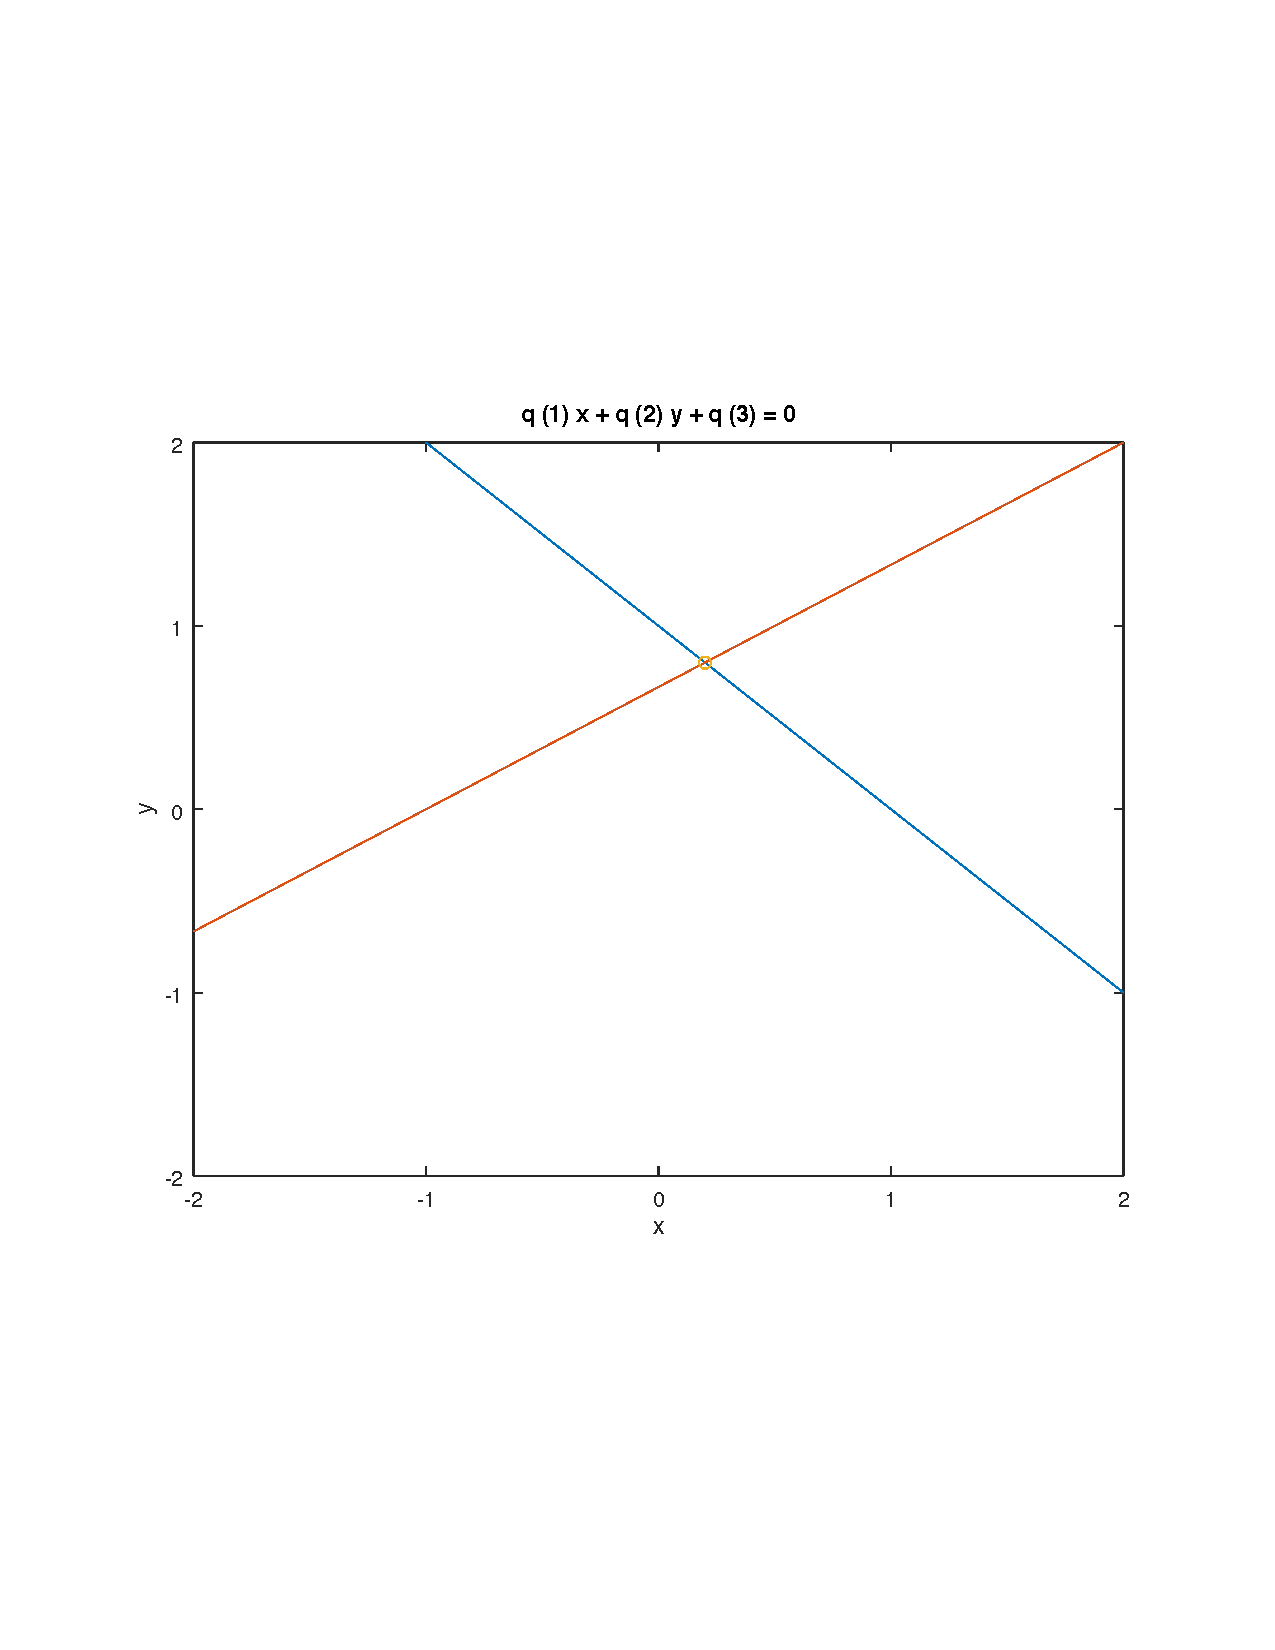
\includegraphics[width=10cm]{slika.pdf}
	\caption{Presek premic $p : x + y - 1 = 0$ in $q : 2x - 3y + 2 = 0$.}
	\label{slika:presek_premic}
\end{figure}
%Koda funkcije presecisce.m.
\lstinputlisting[firstline=1, lastline=17]{presecisce.m}
\end{document}